\documentclass{article}

% Packages required to support encoding
\usepackage{ucs}
\usepackage[utf8x]{inputenc}
\usepackage{graphicx} 
% Packages required by code

% Packages always used
\usepackage{listings}
\usepackage{hyperref}
\usepackage{xspace}
\usepackage[usenames,dvipsnames]{color}
\hypersetup{colorlinks=true,urlcolor=blue}


\usepackage[framed,numbered,autolinebreaks,useliterate] {mcode}


\usepackage{geometry}
\geometry{letterpaper,textwidth=350pt,textheight=680pt,tmargin=60pt,
            left=72pt,footskip=24pt,headsep=18pt,headheight=14pt}
\usepackage{amsmath}
\usepackage{amssymb}
\usepackage{textcase}
\usepackage{soul}

\newcommand{\mat}[1]{\boldsymbol{#1}}\renewcommand{\vec}[1]{\boldsymbol{\mathrm{#1}}}
\newcommand{\vecalt}[1]{\boldsymbol{#1}}

\newcommand{\conj}[1]{\overline{#1}}

\newcommand{\normof}[1]{\|#1\|}
\newcommand{\onormof}[2]{\|#1\|_{#2}}

\newcommand{\itr}[2]{#1^{(#2)}}
\newcommand{\itn}[1]{^{(#1)}}

\newcommand{\eps}{\varepsilon}
\newcommand{\kron}{\otimes}

\DeclareMathOperator{\diag}{diag}
\DeclareMathOperator{\trace}{trace}
\DeclareMathOperator{\tvec}{vec}

\newcommand{\prob}{\mathbb{P}}
\newcommand{\probof}[1]{\prob\left\{ #1 \right\}}

\newcommand{\pmat}[1]{\begin{pmatrix} #1 \end{pmatrix}}
\newcommand{\bmat}[1]{\begin{bmatrix} #1 \end{bmatrix}}
\newcommand{\spmat}[1]{\left(\begin{smallmatrix} #1 \end{smallmatrix}\right)}
\newcommand{\sbmat}[1]{\left[\begin{smallmatrix} #1 \end{smallmatrix}\right]}

\newcommand{\RR}{\mathbb{R}}
\newcommand{\CC}{\mathbb{C}}

\providecommand{\eye}{\mat{I}}
\providecommand{\mA}{\ensuremath{\mat{A}}}
\providecommand{\mB}{\ensuremath{\mat{B}}}
\providecommand{\mC}{\ensuremath{\mat{C}}}
\providecommand{\mD}{\ensuremath{\mat{D}}}
\providecommand{\mE}{\ensuremath{\mat{E}}}
\providecommand{\mF}{\ensuremath{\mat{F}}}
\providecommand{\mG}{\ensuremath{\mat{G}}}
\providecommand{\mH}{\ensuremath{\mat{H}}}
\providecommand{\mI}{\ensuremath{\mat{I}}}
\providecommand{\mJ}{\ensuremath{\mat{J}}}
\providecommand{\mK}{\ensuremath{\mat{K}}}
\providecommand{\mL}{\ensuremath{\mat{L}}}
\providecommand{\mM}{\ensuremath{\mat{M}}}
\providecommand{\mN}{\ensuremath{\mat{N}}}
\providecommand{\mO}{\ensuremath{\mat{O}}}
\providecommand{\mP}{\ensuremath{\mat{P}}}
\providecommand{\mQ}{\ensuremath{\mat{Q}}}
\providecommand{\mR}{\ensuremath{\mat{R}}}
\providecommand{\mS}{\ensuremath{\mat{S}}}
\providecommand{\mT}{\ensuremath{\mat{T}}}
\providecommand{\mU}{\ensuremath{\mat{U}}}
\providecommand{\mV}{\ensuremath{\mat{V}}}
\providecommand{\mW}{\ensuremath{\mat{W}}}
\providecommand{\mX}{\ensuremath{\mat{X}}}
\providecommand{\mY}{\ensuremath{\mat{Y}}}
\providecommand{\mZ}{\ensuremath{\mat{Z}}}
\providecommand{\mLambda}{\ensuremath{\mat{\Lambda}}}
\providecommand{\mPbar}{\bar{\mP}}

\providecommand{\ones}{\vec{e}}
\providecommand{\va}{\ensuremath{\vec{a}}}
\providecommand{\vb}{\ensuremath{\vec{b}}}
\providecommand{\vc}{\ensuremath{\vec{c}}}
\providecommand{\vd}{\ensuremath{\vec{d}}}
\providecommand{\ve}{\ensuremath{\vec{e}}}
\providecommand{\vf}{\ensuremath{\vec{f}}}
\providecommand{\vg}{\ensuremath{\vec{g}}}
\providecommand{\vh}{\ensuremath{\vec{h}}}
\providecommand{\vi}{\ensuremath{\vec{i}}}
\providecommand{\vj}{\ensuremath{\vec{j}}}
\providecommand{\vk}{\ensuremath{\vec{k}}}
\providecommand{\vl}{\ensuremath{\vec{l}}}
\providecommand{\vm}{\ensuremath{\vec{l}}}
\providecommand{\vn}{\ensuremath{\vec{n}}}
\providecommand{\vo}{\ensuremath{\vec{o}}}
\providecommand{\vp}{\ensuremath{\vec{p}}}
\providecommand{\vq}{\ensuremath{\vec{q}}}
\providecommand{\vr}{\ensuremath{\vec{r}}}
\providecommand{\vs}{\ensuremath{\vec{s}}}
\providecommand{\vt}{\ensuremath{\vec{t}}}
\providecommand{\vu}{\ensuremath{\vec{u}}}
\providecommand{\vv}{\ensuremath{\vec{v}}}
\providecommand{\vw}{\ensuremath{\vec{w}}}
\providecommand{\vx}{\ensuremath{\vec{x}}}
\providecommand{\vy}{\ensuremath{\vec{y}}}
\providecommand{\vz}{\ensuremath{\vec{z}}}
\providecommand{\vpi}{\ensuremath{\vecalt{\pi}}}

\sodef\allcapsspacing{\upshape}{0.15em}{0.65em}{0.6em}%

\makeatletter
\def\maketitle{%
\par
\hrule height 0.75pt\vspace{1ex}
\par\noindent
\begin{minipage}{0.5\textwidth}
\scshape
purdue university $\cdot$ CS 580 \\
Introduction to the Analysis of Algorithms
\end{minipage}
\begin{minipage}{0.5\textwidth}
\raggedleft
\MakeTextUppercase{\allcapsspacing{\@title}}\\[0.2ex]
\textit{\@author}\\[0.2ex]
\textit{\@date}
\end{minipage}
\par\vspace{1ex}
\hrule height 1pt
\vspace{2ex}
\par
}
\makeatother

\author{Jun Cheng}
\title{Lecture Notes}
% auto generate a title
\AtBeginDocument{\maketitle}


\title{Homework}





\begin{document} 

\hypertarget{}{}
\subsection*{{Problem 1: }}
\label{}


\begin{figure}[h]
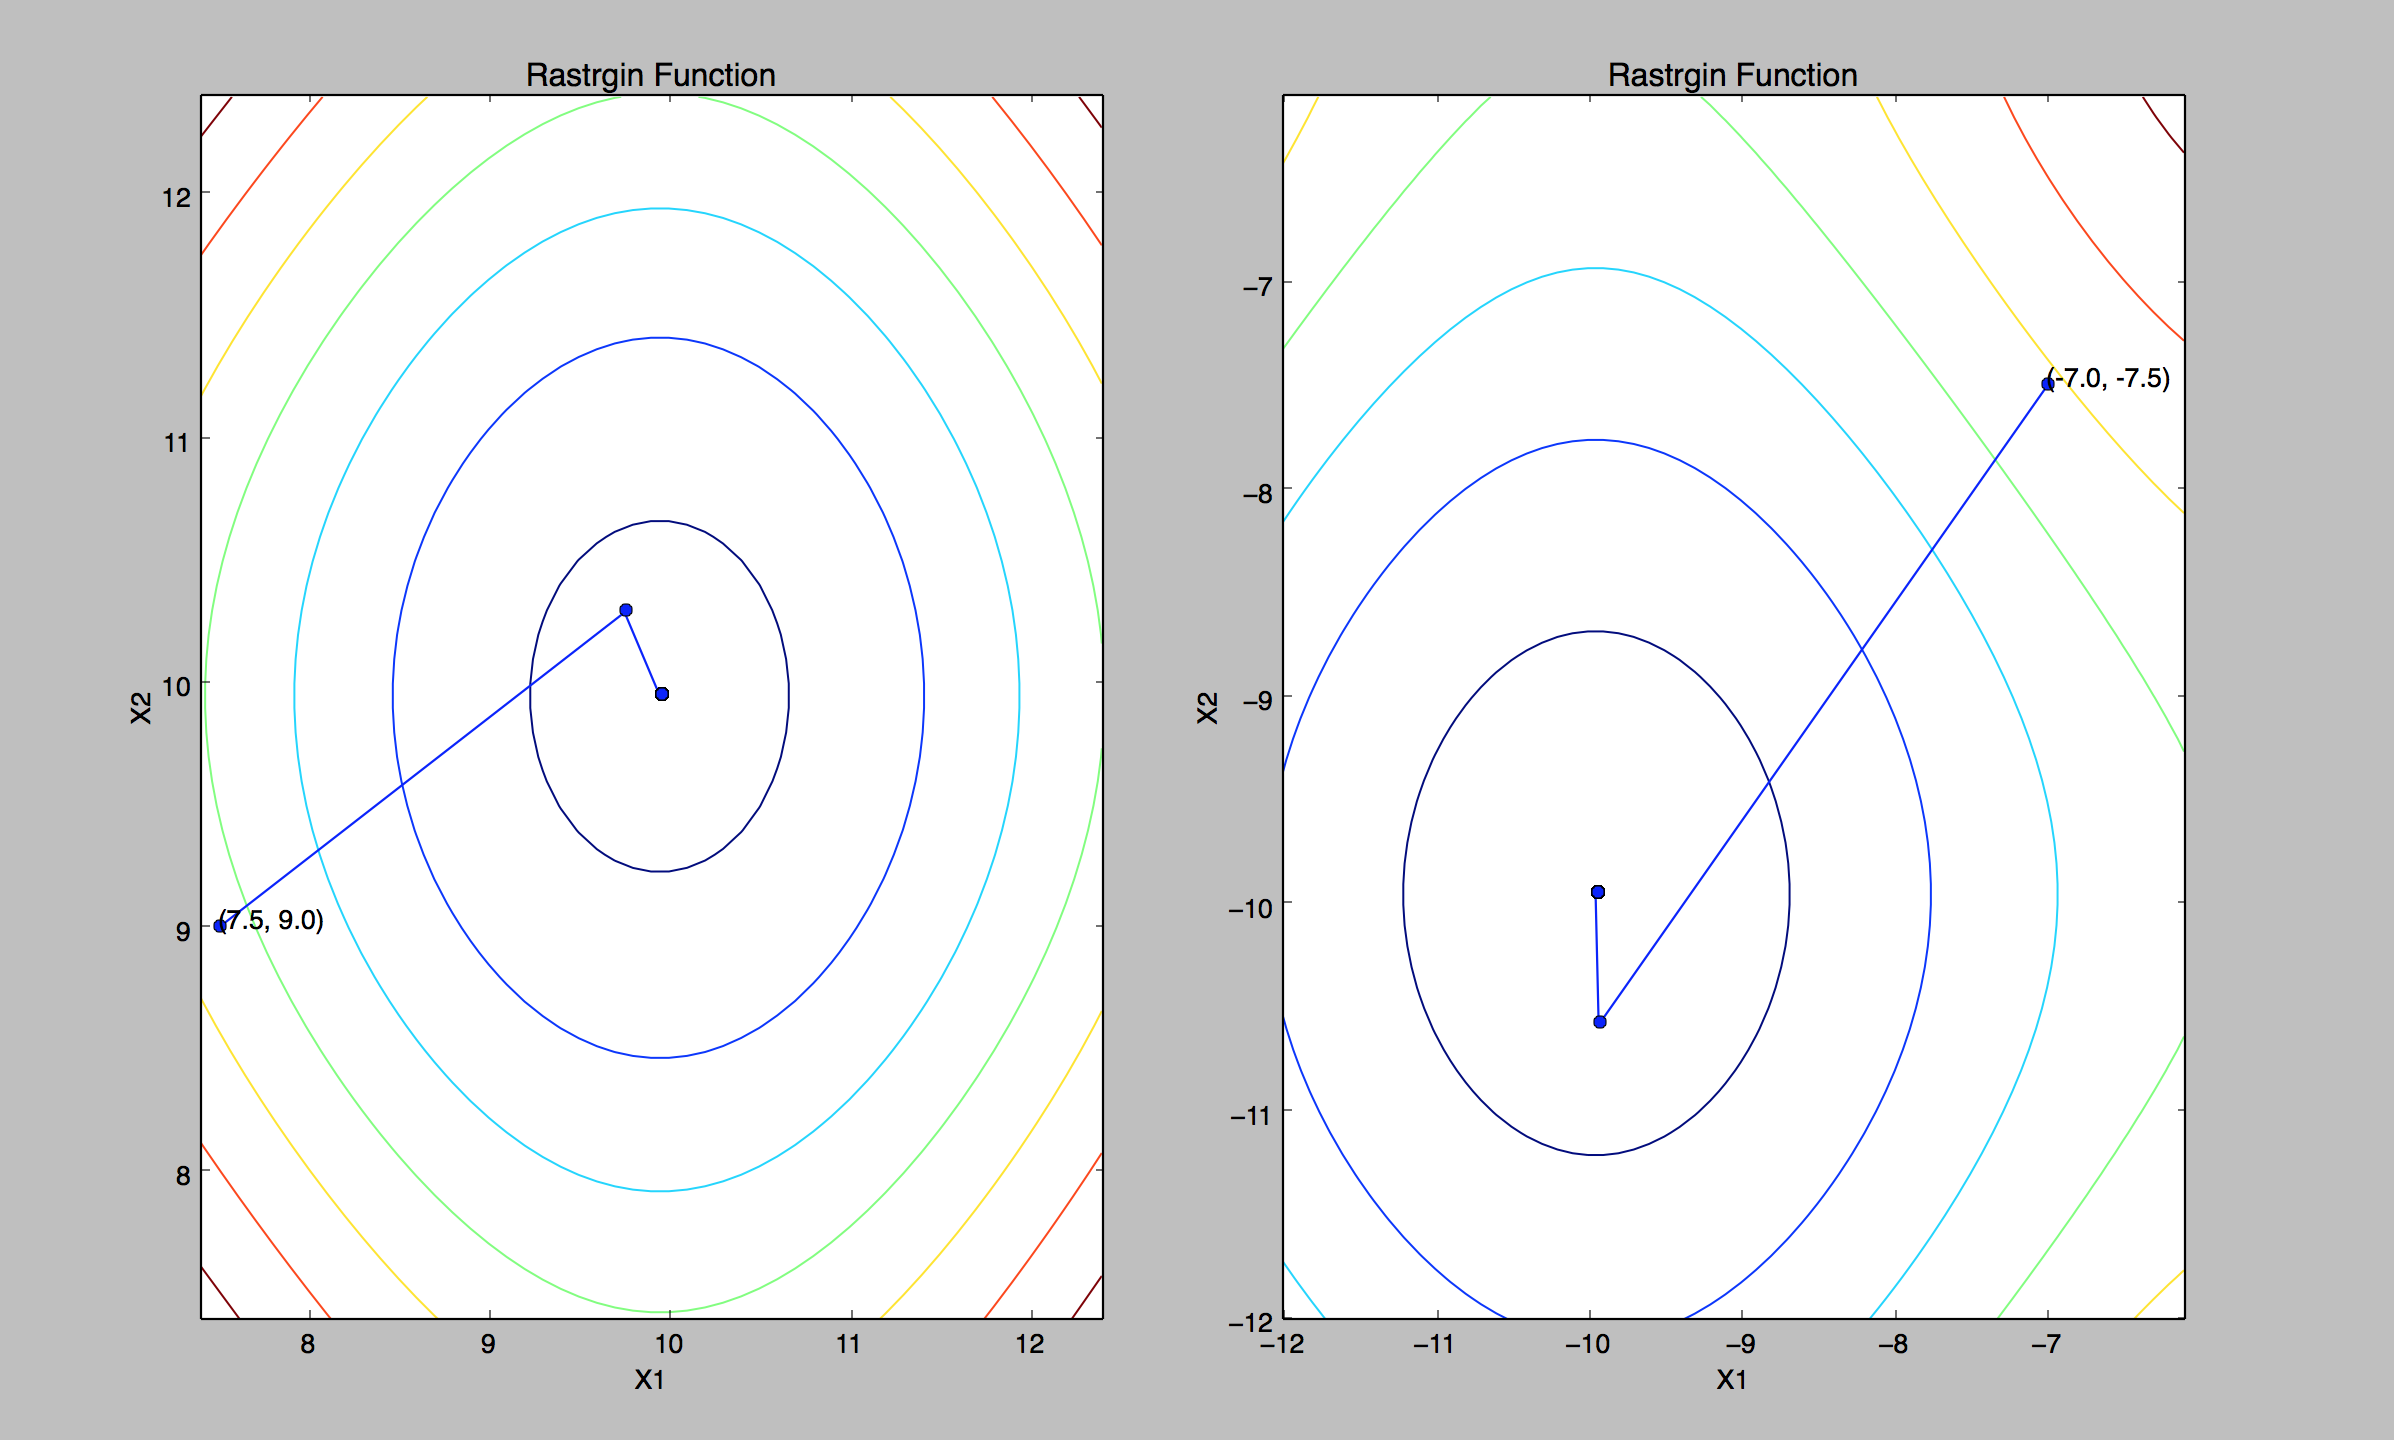
\includegraphics[width=\textwidth]{image/steepest_descent}
\centering
\caption{Steepest descent method. }
\end{figure} 

\begin{figure}[h]
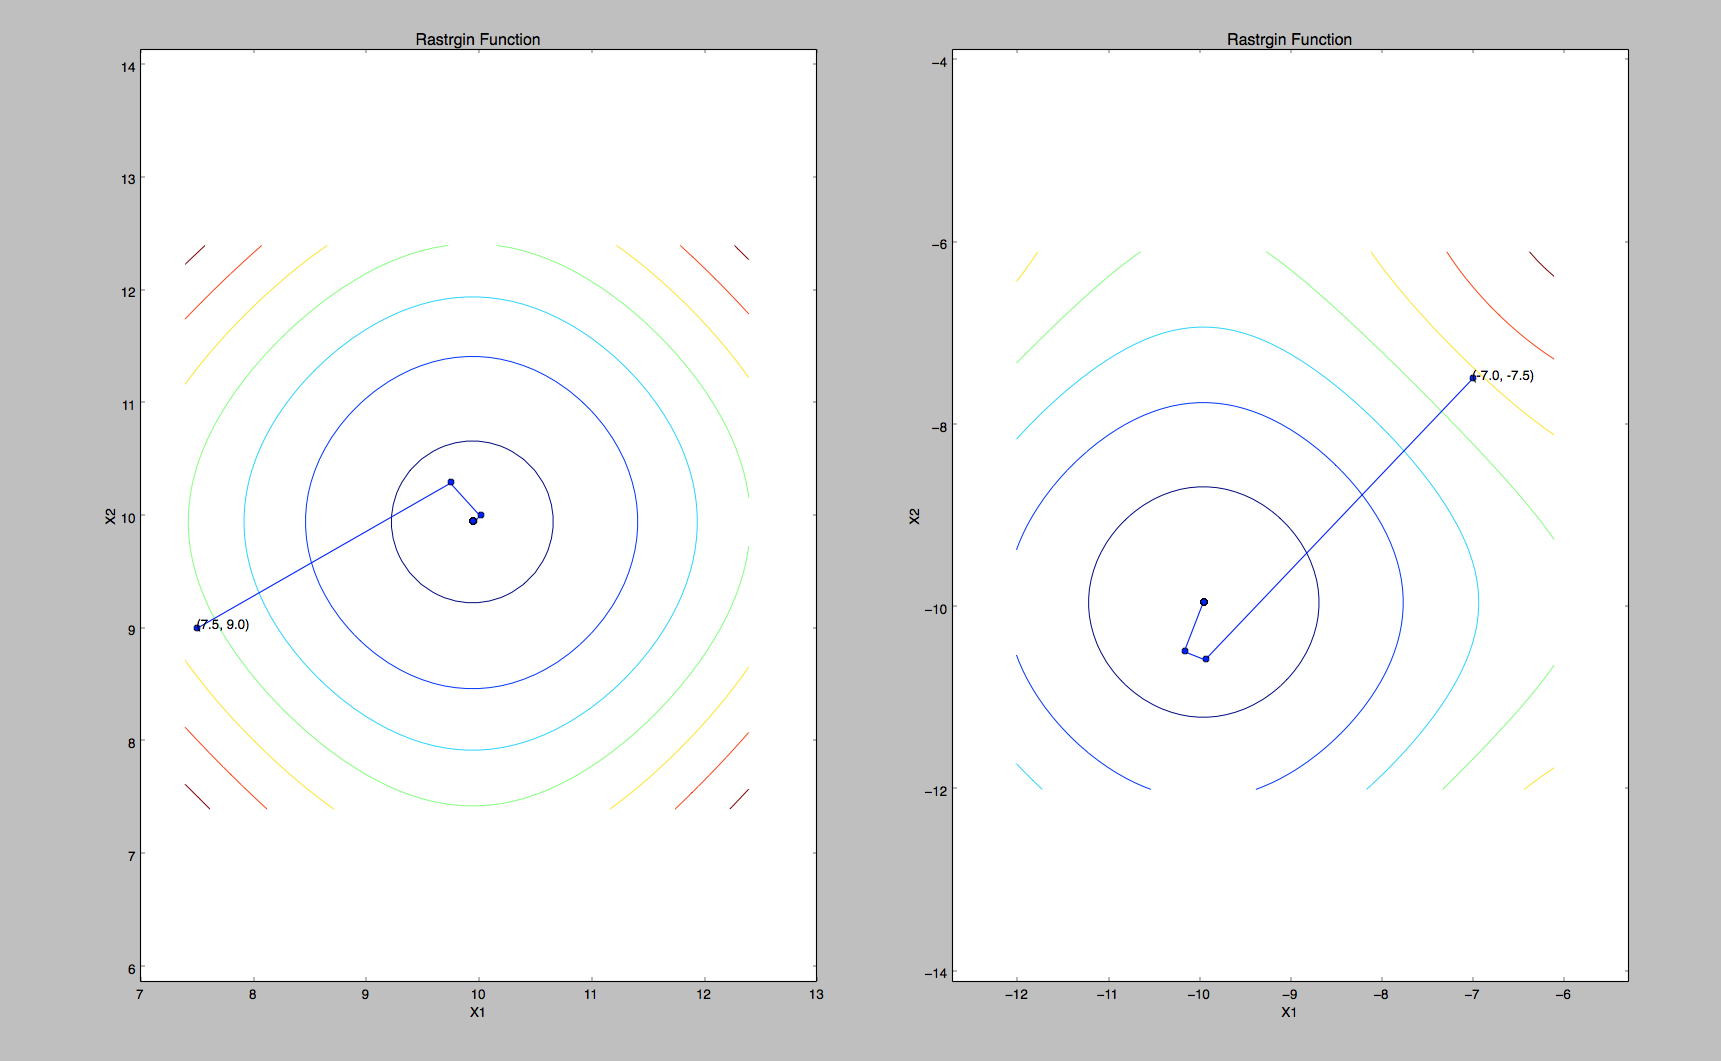
\includegraphics[width=\textwidth]{image/conjugate_gradient}
\centering
\caption{Conjugate gradient method. }
\end{figure} 

\begin{figure}[h]
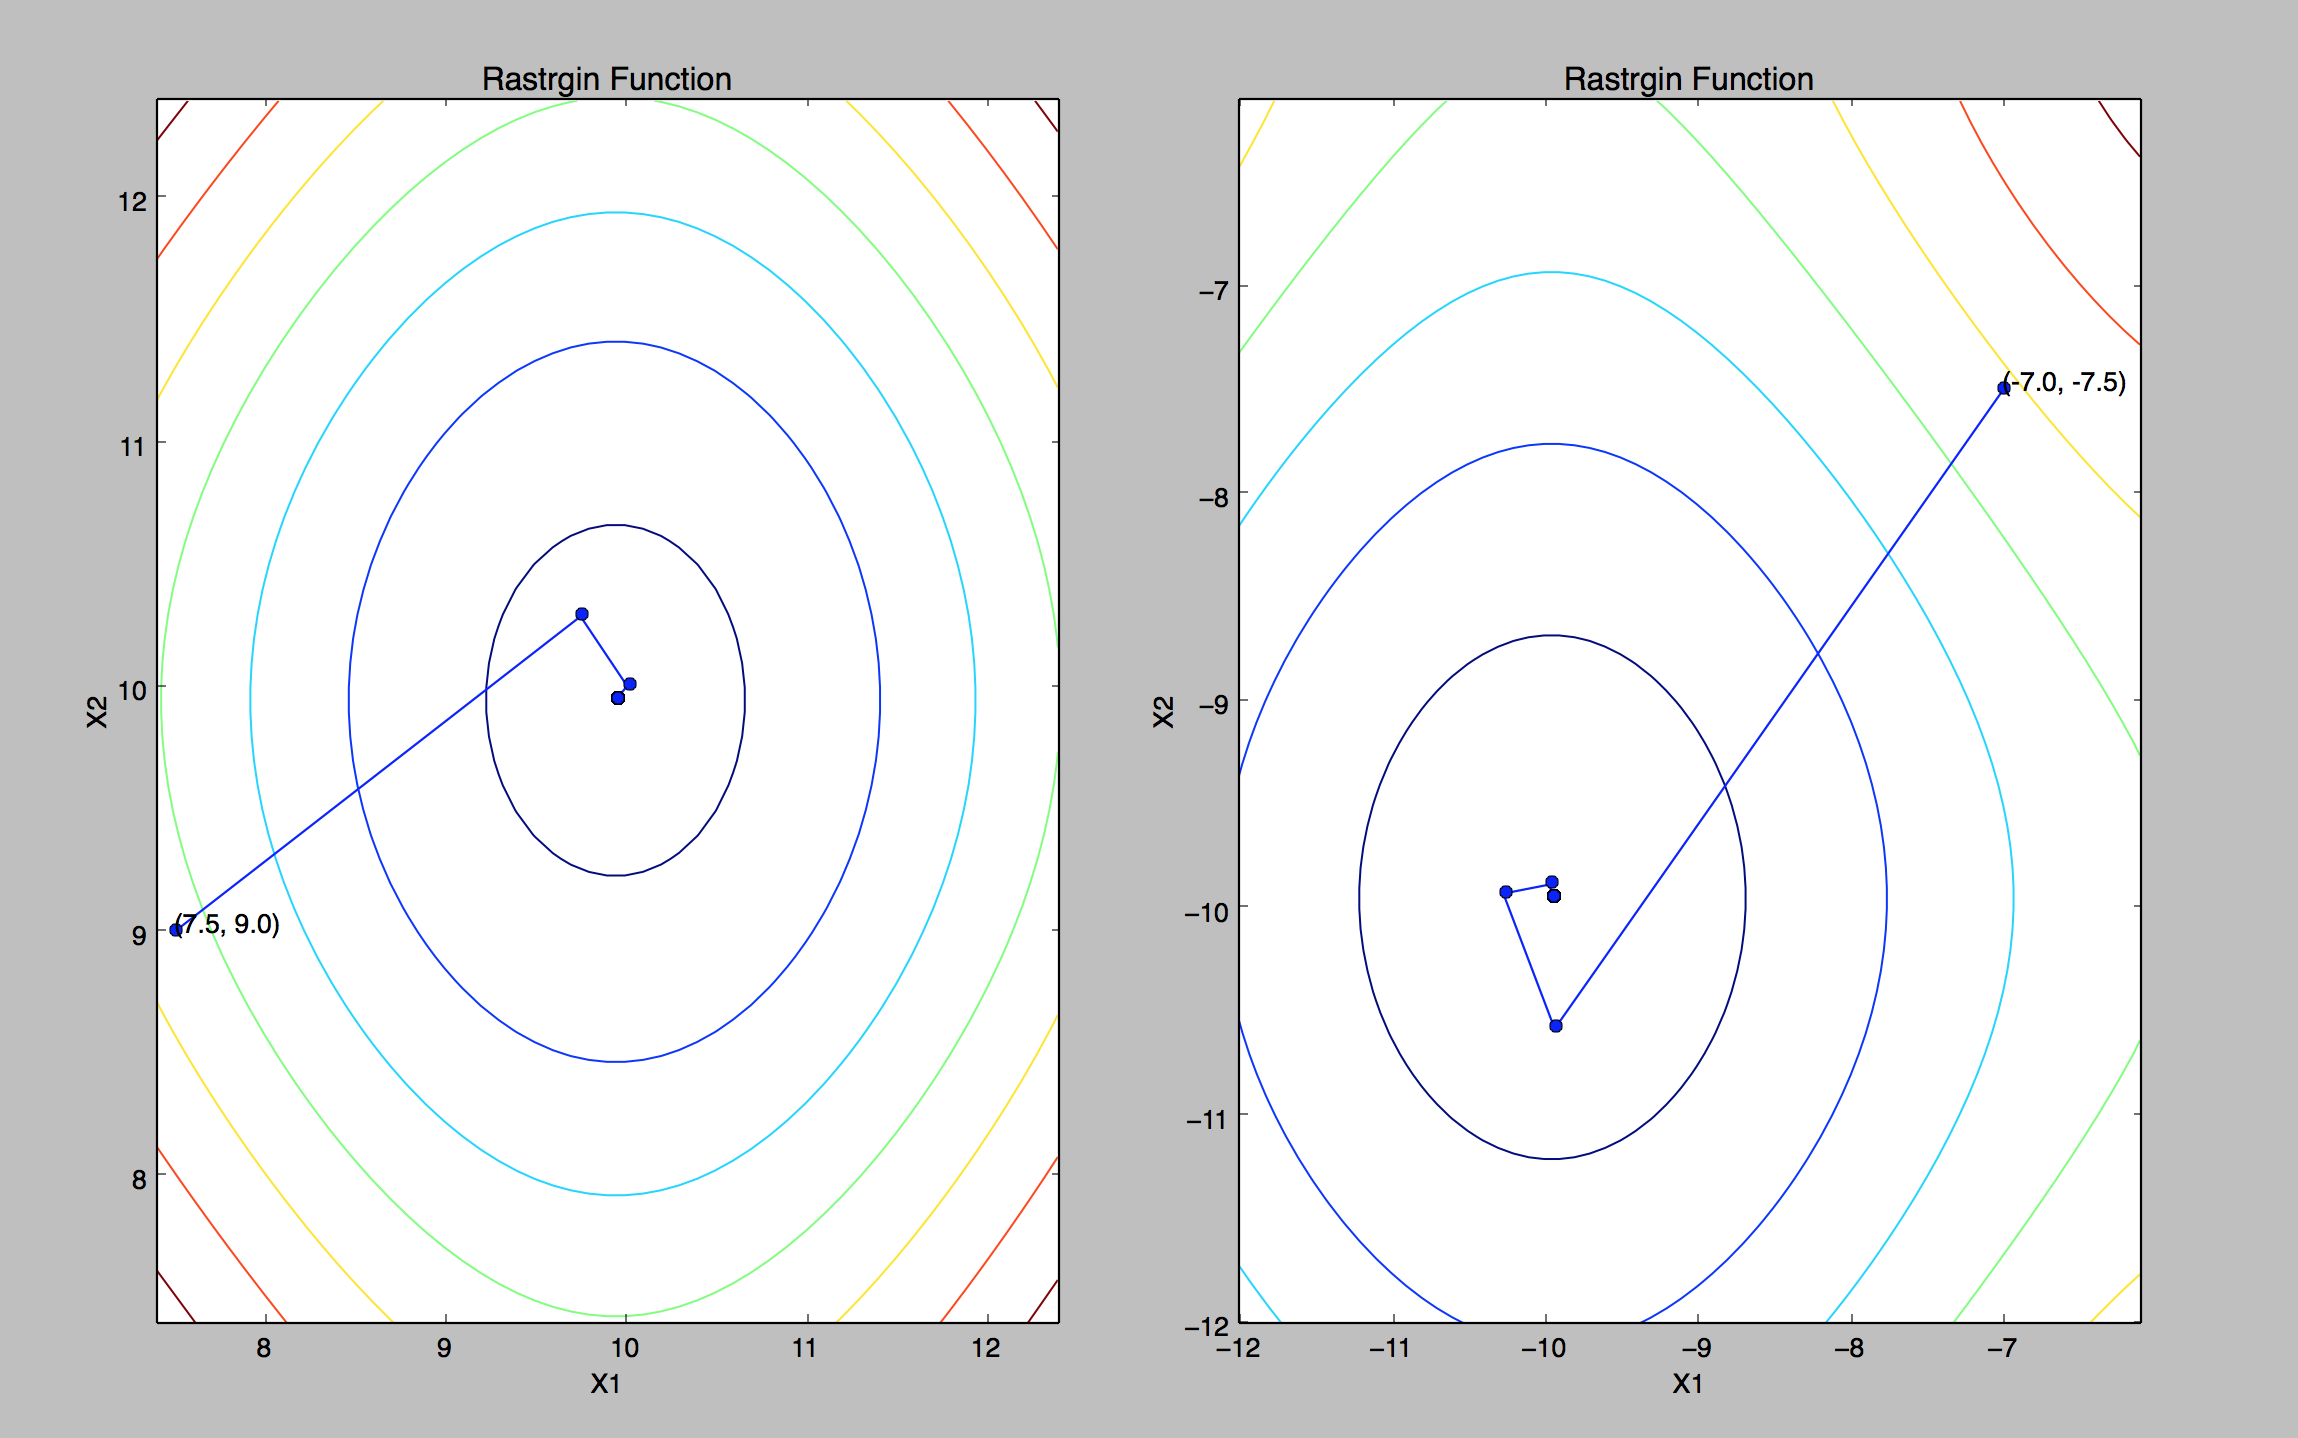
\includegraphics[width=\textwidth]{image/rankone_method}
\centering
\caption{Rank one correction}
\end{figure} 

\begin{figure}[h]
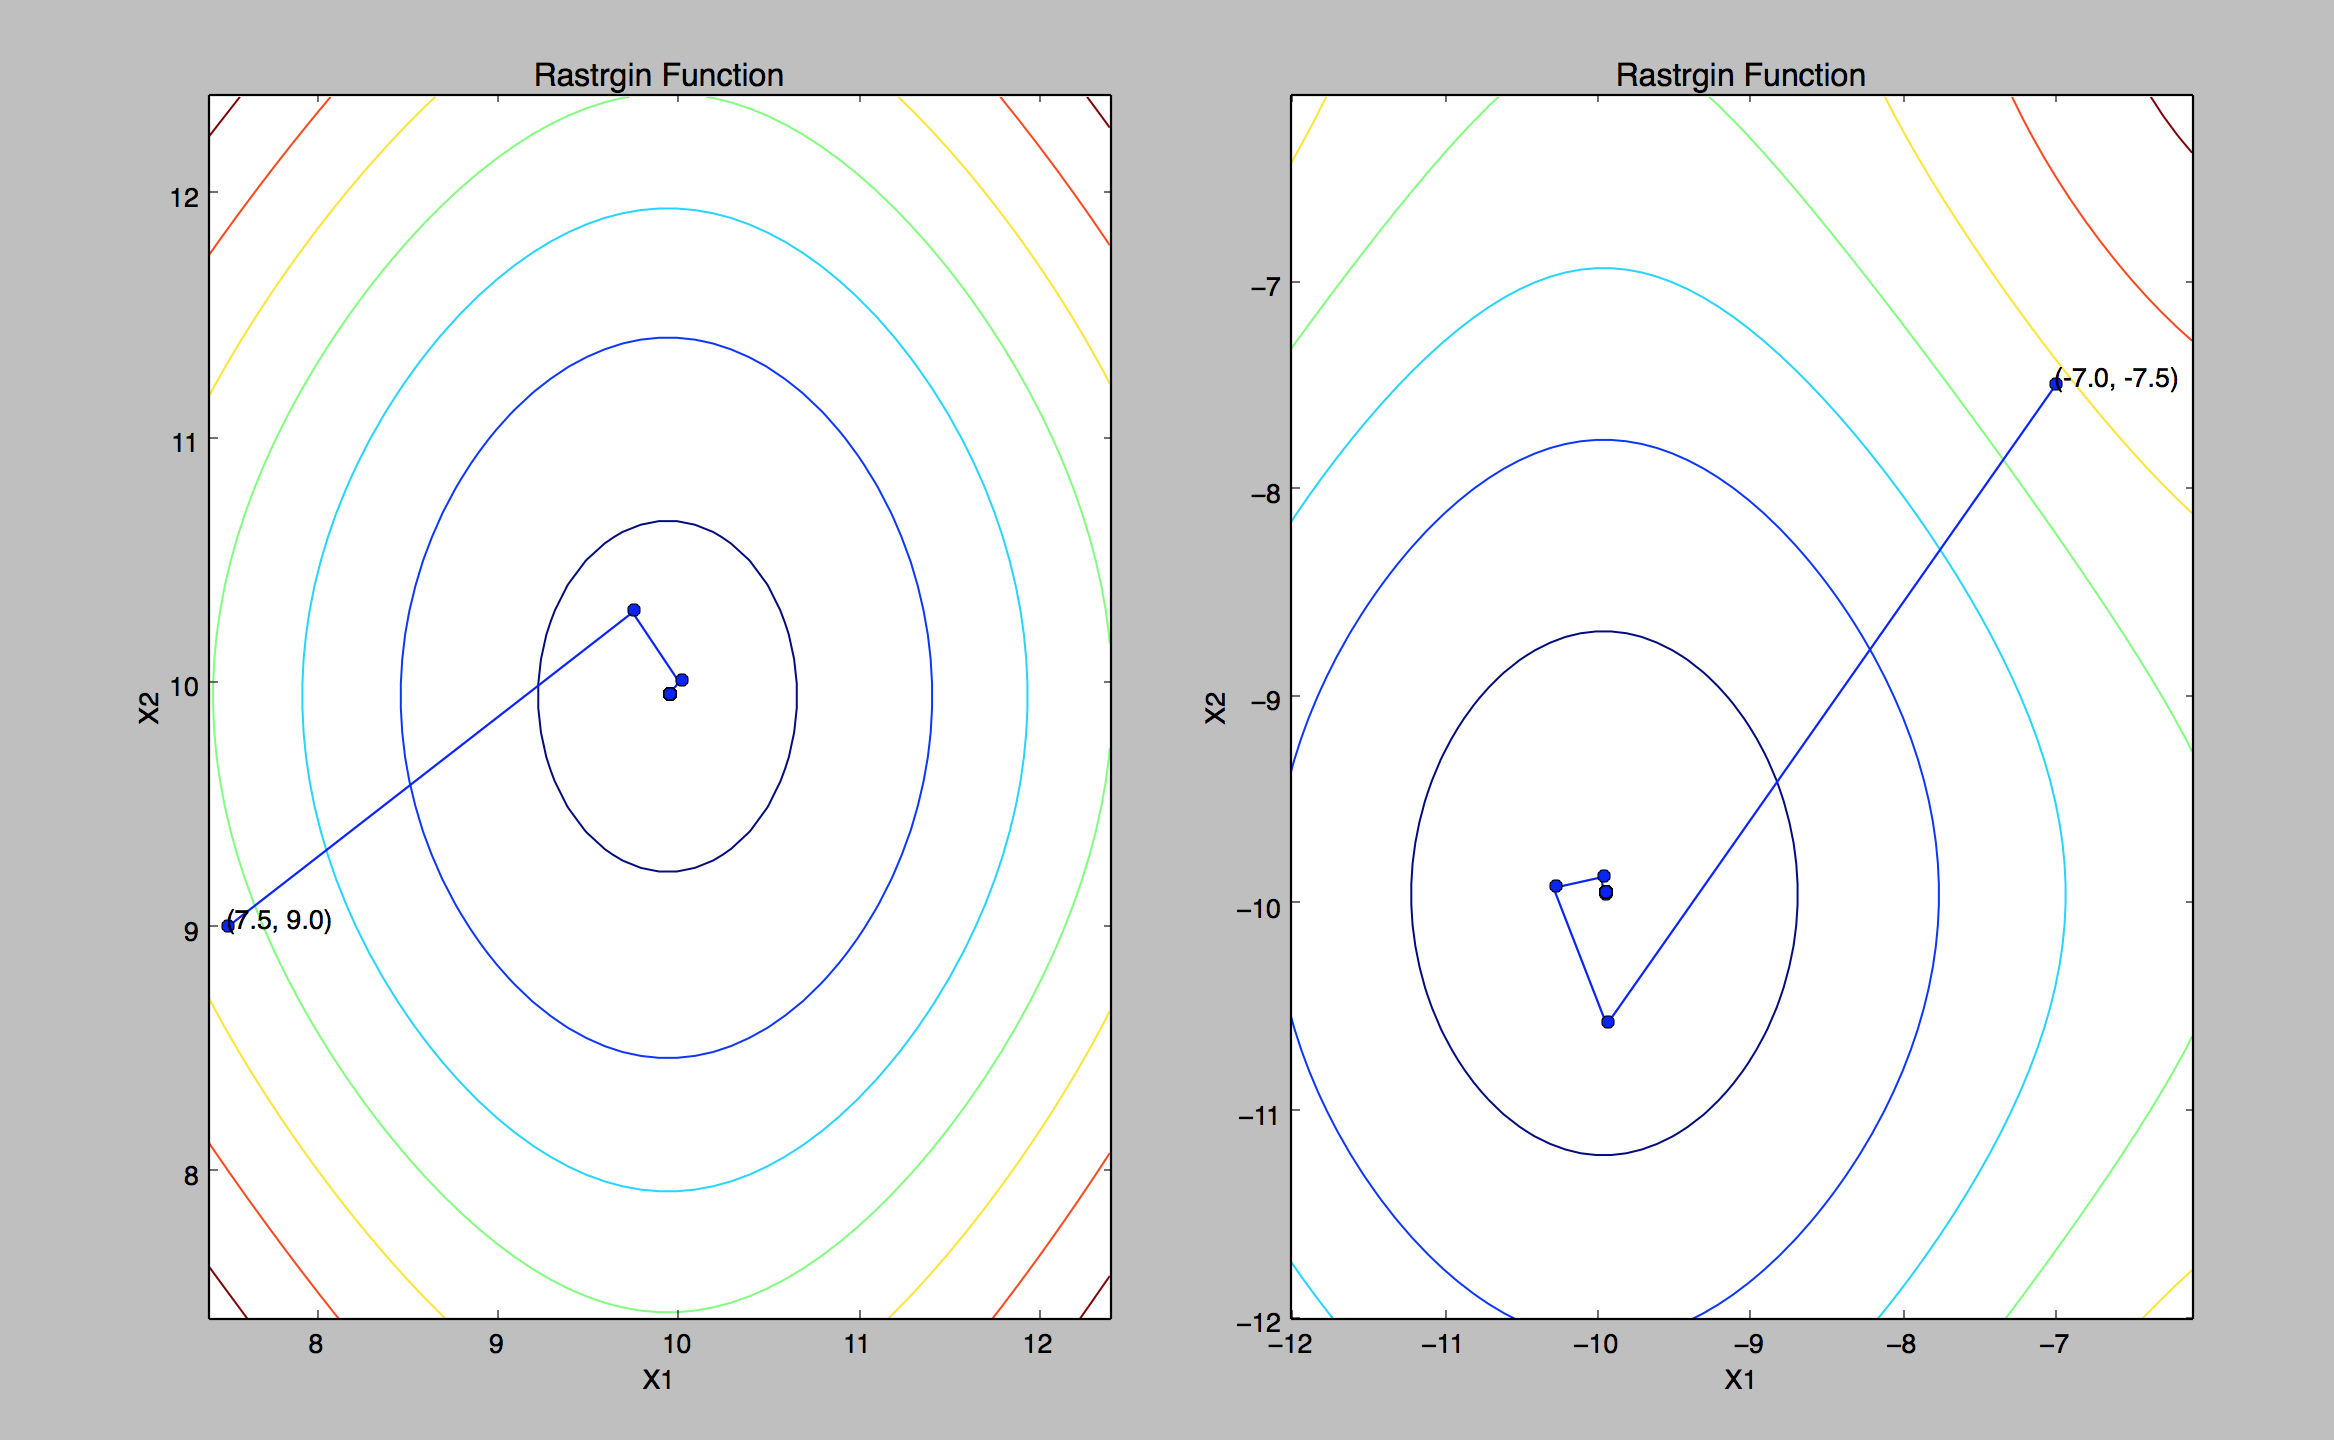
\includegraphics[width=\textwidth]{image/DFP_method}
\centering
\caption{DFP method.   } 
\end{figure} 

\begin{figure}[h]
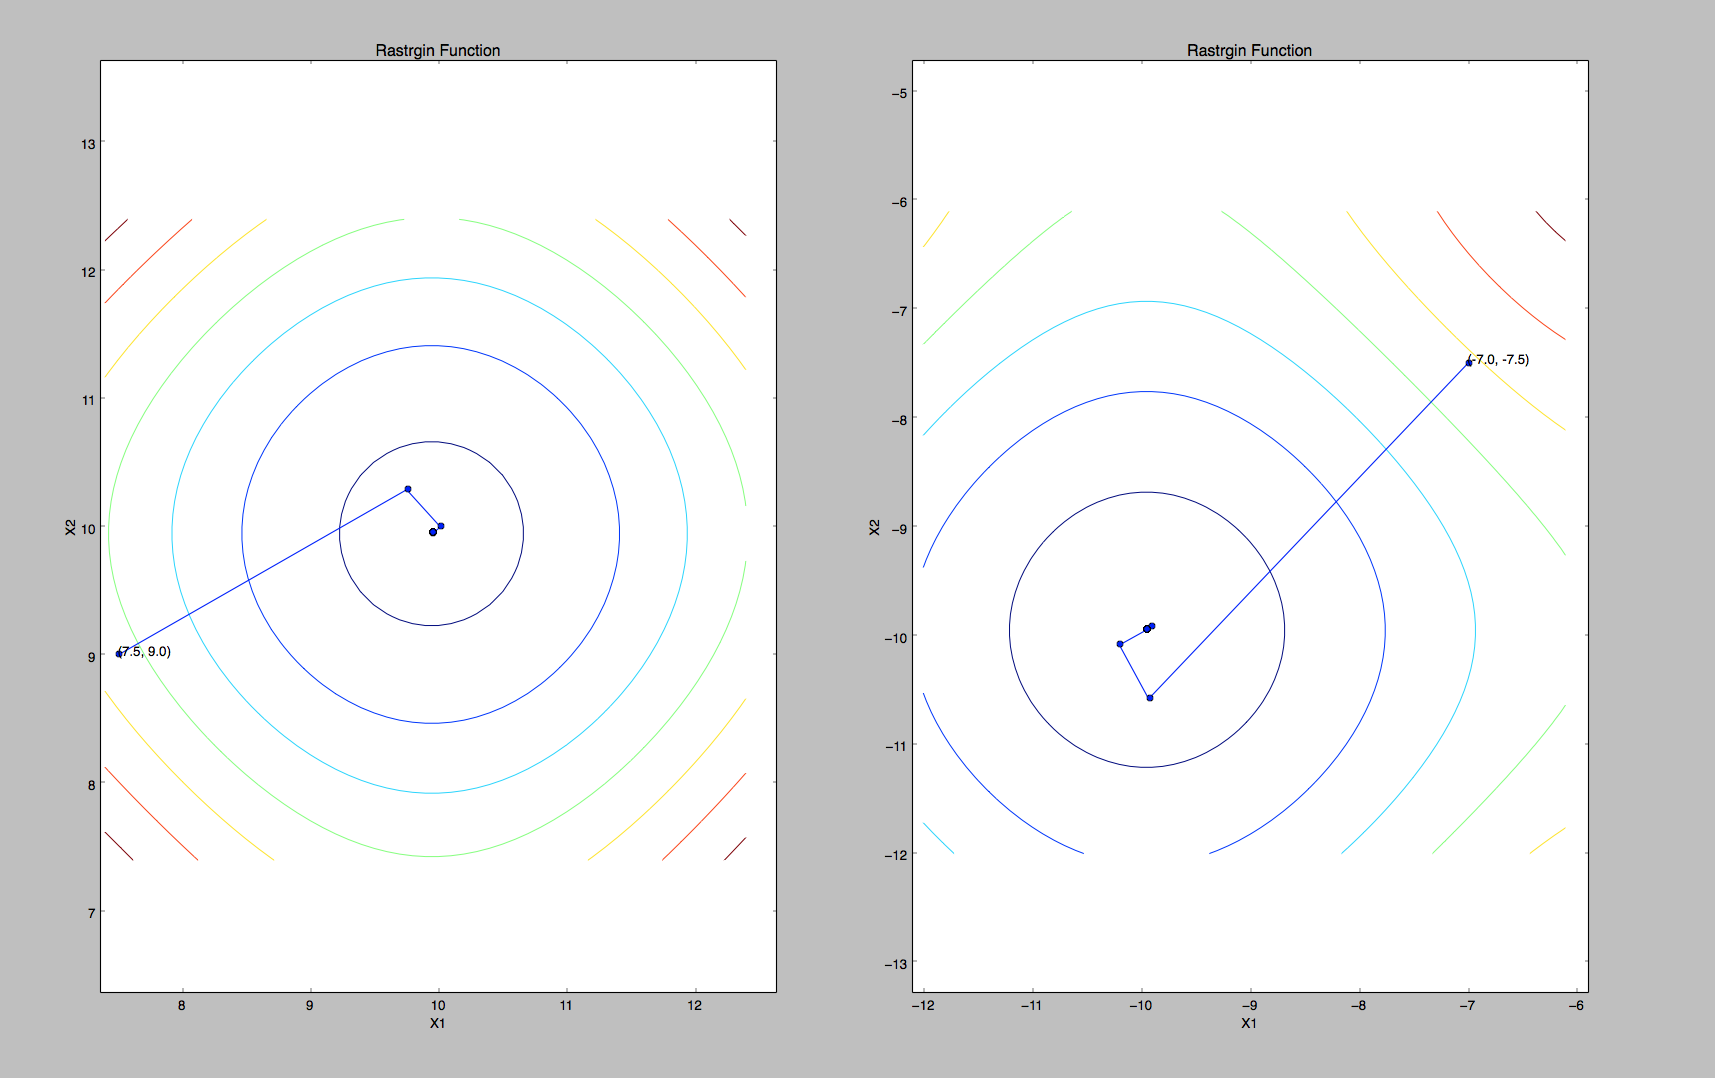
\includegraphics[width=\textwidth]{image/BFGS_method}
\centering
\caption{BFGS method. }
\end{figure} 

\clearpage

\begin{table}[h]
\centering
\caption{Minimization result summary for Rastrigin's function with different starting points }
\label{my-label}
\begin{tabular}{|c|l|l|}
\hline
\textbf{Method}              & \multicolumn{1}{c|}{\textbf{$X_0$: {[}7.5,9.0{]}}} & \multicolumn{1}{c|}{\textbf{$X_0$: {[}-7.0,-7.5{]}}} \\ \hline
\textbf{Steepest Gradient}   & {[}9.94958639528, 9.94958638731{]}                & {[}-9.94958637149, -9.9495863764{]}                 \\ \hline
\textbf{Conjugate Gradient}  & {[}9.94958638332, 9.94958640373{]}                & {[}-9.94958637058, -9.94958637687{]}                \\ \hline
\textbf{Rank one correction} & {[}9.94958641809, 9.94958633077{]}                & {[}-9.94958632695, -9.9495867058{]}                 \\ \hline
\textbf{DFP}                 & {[}9.94958641892, 9.94958632983{]}                & {[}-9.94958638618, -9.94958631318{]}                \\ \hline
\textbf{BFGS}                & {[}9.94958635865, 9.94958639946{]}                & {[}-9.94958647941, -9.94958646598{]}                \\ \hline
\end{tabular}
\end{table}

\\
Code (python):  \\
\begin{lstlisting} 

import matplotlib.pyplot as plt

import numpy as np
def rastriginFunc(x1, x2):
    return 20 + 0.01*x1**2 + 0.01*x2**2 \
           - 10*(np.cos(0.2*np.pi*x1)+np.cos(0.2*np.pi*x2))


def plotContour(ax, xlim, ylim):
    delta = 0.1
    x = np.arange(xlim[0], xlim[1], delta)
    y = np.arange(ylim[0], ylim[1], delta)
    X1, X2 = np.meshgrid(x, y)
    Z = rastriginFunc(X1,X2)
    ax.set_title("Rastrgin Function")
    ax.set_xlabel("X1")
    ax.set_ylabel("X2")
    cs = ax.contour(X1, X2, Z)
    return cs

def gradientRastrigin(x1, x2):
    # df/dx1:
    g1 = 0.02*x1 +2*np.pi*np.sin(0.2*np.pi*x1)
    g2 = 0.02*x2 +2*np.pi*np.sin(0.2*np.pi*x2)
    return g1, g2


def lineSearchFunc(X, alpha, D):
    x1, x2 = X
    d1, d2 = D
    return rastriginFunc(x1 + alpha * d1, x2 + alpha * d2)

def goldenSection(func, X, Direction,  left ,right, tol):
    rho = (np.sqrt(5)-1)/2  # 1.618
    length = right - left
    if abs(length) < tol:
        return (right + left)/2
    mR = left  +  rho * length
    mL = right -  rho * length

    if func(X, mL,Direction ) < func( X, mR, Direction):
        return goldenSection(func,X, Direction,  left, mR,tol)
    else:
        return goldenSection(func,X, Direction,  mL, right, tol)



def bracket(Alpha0, func, X, D, epsilon):

    Xleft = Alpha0
    Xright = 0
    i = 1
    while i<100:     ## i can not be too large.
        Xright += Xleft + i* epsilon
        #print Xright, func(X, Xright, D)
        if func(X, Xright, D) >= func(X, Xleft, D):
            return Xleft, Xright
        else:
            i+=1
            Xleft = Xright


def steepesDescent(X0, tol):
    x1List = []
    x2List = []
    x1_current = X0[0]
    x2_current = X0[1]
    g1, g2 = 1.0, 1.0
    counter = 0 
    while np.sqrt(g1**2 + g2**2) > tol:
        x1List.append(x1_current)
        x2List.append(x2_current)
        #print x1_current, x2_current
        g1, g2 = gradientRastrigin(x1_current, x2_current)
        iLeft, iRight = bracket(0, lineSearchFunc, (x1_current, x2_current), (-g1, -g2), epsilon=0.001)
        alpha = goldenSection(lineSearchFunc,(x1_current, x2_current),(-g1, -g2), iLeft, iRight, tol)
        x1_current = x1_current - alpha * g1
        x2_current = x2_current - alpha * g2
        counter += 1
        if counter>100:
            print "Iteration more than 100"
            break


    return x1List, x2List


def conjugateGradient(X0, tol) :
    x1List = []
    x2List = []
    x1_current = X0[0]
    x2_current = X0[1]
    g1, g2 = gradientRastrigin(x1_current, x2_current)
    d1, d2 = -g1, -g2
    counter = 0
    while np.sqrt(g1**2 + g2**2) > tol: # and counter < 10:
        x1List.append(x1_current)
        x2List.append(x2_current)
        #print x1_current, x2_current
        g1, g2 = gradientRastrigin(x1_current, x2_current)
        iLeft, iRight = bracket(0, lineSearchFunc, (x1_current, x2_current), (d1, d2), epsilon=0.001)
        alpha = goldenSection(lineSearchFunc,(x1_current, x2_current),(d1, d2), iLeft, iRight, tol)

        x1_current = x1_current + alpha * d1
        x2_current = x2_current + alpha * d2

        g1_new, g2_new = gradientRastrigin(x1_current, x2_current)
        beta = max(0, (g1_new*(g1_new - g1) + g2_new*(g2_new-g2))/(g1*g1 + g2*g2) )
        d1 = -g1_new + beta * d1
        d2 = -g2_new + beta * d2

        
        counter += 1
        if counter>100:
            print "Iteration more than 100"
            break
    return x1List, x2List

def rankone(X0, tol):

    x1List = []
    x2List = []
    x1_current = X0[0]
    x2_current = X0[1]
    g1, g2 = gradientRastrigin(x1_current, x2_current)
    H = np.identity(2)
    D =-H * np.matrix([[g1], [g2]])
    d1, d2 = D.tolist()[0][0], D.tolist()[1][0]
    counter = 0 
    while np.sqrt(g1**2 + g2**2) > tol: # and counter < 100:
        x1List.append(x1_current)
        x2List.append(x2_current)
        #print x1_current, x2_current
        g1, g2 = gradientRastrigin(x1_current, x2_current)
        iLeft, iRight = bracket(0, lineSearchFunc, (x1_current, x2_current), (d1, d2), epsilon=0.001)
        alpha = goldenSection(lineSearchFunc,(x1_current, x2_current),(d1, d2), iLeft, iRight, tol)



        x1_current = x1_current + alpha * d1
        x2_current = x2_current + alpha * d2

        g1_new, g2_new = gradientRastrigin(x1_current, x2_current)
        diff_x = alpha * np.matrix([[d1], [d2]])
        diff_g = np.matrix([[g1_new-g1], [g2_new-g2]])
        denom =np.dot( diff_g.transpose(), (diff_x - H*diff_g)).tolist()[0][0]
        numerator = (diff_x - H*diff_g)*((diff_x - H*diff_g).transpose())
        H =  H + 1.0/denom*numerator
        D = -H* np.matrix([[g1_new], [g2_new]])
        d1, d2 = D.tolist()[0][0], D.tolist()[1][0]

        counter += 1
        if counter>100:
            print "Iteration more than 100"
            break


    return x1List, x2List

def DFP(X0, tol):

    x1List = []
    x2List = []
    x1_current = X0[0]
    x2_current = X0[1]
    g1, g2 = gradientRastrigin(x1_current, x2_current)
    H = np.identity(2)
    D =-H * np.matrix([[g1], [g2]])
    d1, d2 = D.tolist()[0][0], D.tolist()[1][0]
    counter = 0
    while np.sqrt(g1**2 + g2**2) > tol: # and counter < 100:
        x1List.append(x1_current)
        x2List.append(x2_current)
        #print x1_current, x2_current
        g1, g2 = gradientRastrigin(x1_current, x2_current)
        iLeft, iRight = bracket(0, lineSearchFunc, (x1_current, x2_current), (d1, d2), epsilon=0.001)
        alpha = goldenSection(lineSearchFunc,(x1_current, x2_current),(d1, d2), iLeft, iRight, tol)



        x1_current = x1_current + alpha * d1
        x2_current = x2_current + alpha * d2

        g1_new, g2_new = gradientRastrigin(x1_current, x2_current)
        diff_x = alpha * np.matrix([[d1], [d2]])
        diff_g = np.matrix([[g1_new-g1], [g2_new-g2]])
        denom1 = np.dot(diff_x.transpose(), diff_g).tolist()[0][0]
        numerator1 = diff_x * (diff_x.transpose())

        denom2 =np.dot( diff_g.transpose(), H*diff_g).tolist()[0][0]
        numerator2 = (H*diff_g)*((H*diff_g).transpose())
        H =  H + numerator1/denom1 - numerator2/denom2  #denom*numerator
        D = -H* np.matrix([[g1_new], [g2_new]])
        d1, d2 = D.tolist()[0][0], D.tolist()[1][0]

        counter += 1
        if counter>100:
            print "Iteration more than 100"
            break

    return x1List, x2List

def BFGS(X0, tol):

    x1List = []
    x2List = []
    x1_current = X0[0]
    x2_current = X0[1]
    g1, g2 = gradientRastrigin(x1_current, x2_current)
    H = np.identity(2)
    D =-H * np.matrix([[g1], [g2]])
    d1, d2 = D.tolist()[0][0], D.tolist()[1][0]
    counter = 0
    while np.sqrt(g1**2 + g2**2) > tol:
        x1List.append(x1_current)
        x2List.append(x2_current)
        #print x1_current, x2_current
        g1, g2 = gradientRastrigin(x1_current, x2_current)
        iLeft, iRight = bracket(0, lineSearchFunc, (x1_current, x2_current), (d1, d2), epsilon=0.001)
        alpha = goldenSection(lineSearchFunc,(x1_current, x2_current),(d1, d2), iLeft, iRight, tol)



        x1_current = x1_current + alpha * d1
        x2_current = x2_current + alpha * d2

        g1_new, g2_new = gradientRastrigin(x1_current, x2_current)
        diff_x = alpha * np.matrix([[d1], [d2]])
        diff_g = np.matrix([[g1_new-g1], [g2_new-g2]])

        denom0      =   np.dot(diff_g.transpose(), diff_x).tolist()[0][0]
        numerator0  =   np.dot(diff_g.transpose(), H*diff_g).tolist()[0][0]


        denom1      = np.dot(diff_x.transpose(), diff_g)
        numerator1  = diff_x * (diff_x.transpose())
        denom2 =np.dot( diff_g.transpose(), diff_x).tolist()[0][0]
        numerator2 = H*diff_g*(diff_x.transpose()) + (H*diff_g*(diff_x.transpose())).transpose()

        H =  H + (1+numerator0/denom0)*numerator1/denom1 - numerator2/denom2  #denom*numerator

        D = -H* np.matrix([[g1_new], [g2_new]])
        d1, d2 = D.tolist()[0][0], D.tolist()[1][0]
        counter +=  1
        if counter>100:
            print "Iteration more than 100"
            break



    return x1List, x2List



def minfinder(method):

    X0_p= (7.5, 9.0)
    X0_n= (-7.0, -7.5)

    f, (ax1, ax2) = plt.subplots(1,2, sharex=False)
    ## For starting point (7.5, 9.0)
    plotContour(ax1, [7.4,12.5] , [7.4,12.5])
    x1List, x2List = method(X0_p, tol=1.0e-8)
    ax1.annotate('(%s, %s)'% X0_p, xy= X0_p, textcoords='data' )
    ax1.plot(x1List, x2List, 'o-')
    ax1.axis('equal')
    print "[" + str(x1List[-1]) + ", "  + str(x2List[-1]) + "]"

    ## For starting point (-7.0, -7.5)
    plotContour(ax2, [-12.0,-6.00] , [-12.0,-6.0])
    x1List, x2List = method(X0_n, tol=1.0e-8)
    ax2.annotate('(%s, %s)'% X0_n, xy= X0_n, textcoords='data' )
    ax2.plot(x1List, x2List, 'o-')
    ax2.axis('equal')


    print "[" + str(x1List[-1]) + ", "  + str(x2List[-1]) + "]"
    plt.show()

def main():
    #minfinder(method = steepesDescent)
    #minfinder(method = conjugateGradient)
    #minfinder(method=rankone)
    #minfinder(method= DFP)
    minfinder(method=BFGS)

if  __name__ == "__main__":
    main()
\end{lstlisting}




\end{document}
